  % Chapter 4

\chapter{Needs Assessment and Problem Identification } % Main chapter title

\label{Chapter4} % For referencing the chapter elsewhere, use \ref{Chapter4} 

%------------------------------------------------------

\section{Introduction}
In this chapter, we present a contextual inquiry study conducted with mothers of premature infants and Neonatal Intensive Care Unit (NICU) staff (doctors and nurses) at the Groote Schuur Hospital in Cape Town.  The goals of this study were to:
\begin{enumerate}
      \item Observe and familiarize with the NICU environment
       \item Establish a working relationship with mothers and NICU staff
        \item Identify stakeholders' NICU experiences and main challenges that hinders communication in the NICU; and
         \item Understand stakeholder's needs and requirement regarding a  possible solutions that could be used to enhance communication between NICU staff and mothers 
\end{enumerate}

\section{Research Perspective}
In this study, we chose to use a bottom-up user-centric approach \citep{Abras2004, Balaam2015} focusing on conceptualizing the NICU environment to understand the existing workflow, communication problems and design of a possible communication intervention. In this phase, we did not approach the NICU stakeholders with a specific system ideas. Instead, we motivated the stakeholders (nurses, doctors and mothers) to share the challenges they face while taking care of the hospitalized infants and provide suggestions of possible interventions that fit in their socio-economic situation.

We chose to use this approach because it focuses on the explicit understanding of users, tasks, and environments in which they work from~\citep{Abras2004}. In addition, this approach is encouraged health field because it agrees with healthcare institutions/organizations such as the National Academy of Medicine (NAM)\footnote{The National Academy of Medicine (NAM) is one of three academies that make up the National Academies of Sciences, Engineering, and Medicine (the National Academies) in the United States} that advocates for user-centric approach when developing healthcare technologies ~\citep{DeVitoDabbs2009}.  Furthermore, several researchers conducting Information and Communication Technology for Development (ICT4D) projects recommend this approach to improve quality and sustainability of technological solution~\citep{Heeks2008,Pankomera2018, Mukisa2017}.

\textcite{Piper2018} and ~\textcite{Rogers2013} sensitive the importance of understanding the stakeholders context and needs to ensure the designed tool meets the end users needs. However, most healthcare systems designed for developing countries often rely on top-down approach. The ICT4D and Human Computer Interaction for Development (HCI4D) researchers frame the needs of end users with their own theories and ordering and later impose them on the participants. Consequently, this increases the researchers' tendency to designing and developing technological solutions based on their own understanding. ~\textcite{Rogers2013} refers to this approach as designing in "third-person mode". This is a case where the researcher has predefined research needs and goals, therefore imposing them on the participants during the design process. Often, this design process ends up with easy-to-use systems that are usually used in the inception of the system deployment but later the users stop using them.

In the design of health care systems, patients or caregivers involvement: where they share their lived experiences of health and social care; is essential to ensure that the researchers understand not only their system desires but also their feelings and needs. In addition, it help the researcher to utilize patients or caregivers specialist knowledge which in return gives participants a strong voice in how health systems or services should change. This last aspect is essential if changes are to be sustainable in healthcare. Furthermore, previous studies have proved that such participation allows the researcher to build a rapport with the participants which is more important than the designing a system which end users might not relate to \citep{Wolstenholme2017,Nilsson2016,Ward2018}. 

In the same vein, this study focuses on engaging the participants throughout the design process to empower and encourage them to articulate their design needs and ideas. We acknowledge that our stakeholders have limited prior design skills but based on their rich lived NICU experience, they were best placed to design the appropriate technological artifact that could bridge the communication gap in the NICU. On that basis, we did not approach our stakeholders with a defined design idea. Instead we allowed them to lead the co-design process and explore possible technological solution according to the technologies they possessed or had access to. This approach empowered participants to fully engage in the design process, encouraging them to contribute towards the shaping of new technological intervention that could meet their needs in their existing socio-economical condition. We argue that this approach progressively fostered mutual learning  between multiple stakeholders in a hierarchical infant care structure, enabling them to collaborate in identifying most viable technologies that could be used in Groote Schuur Hopital (GSH) NICU context.

In the sections that follow, we discuss the methods used to understand the NICU environment and stakeholders, what we learned and the outcomes of our activities concerning the design of the a possible communication intervention. Since we have not come across existing literature that focus on design on NICU systems in low-income context, we argue that our methodology approach helped us to familiarize and understand the stress related to premature birth and the communication challenges that the NICU staff and mothers face as they partake in the care of the hospitalized infants.

\section{Needs Assessment (Sept 2017- Feb 2018}
The focus  of this phase was to introduce the study to the stakeholders (mothers of premature infants, NICU nurses and doctors), engage them in identifying the common NICU communication challenges and suggestions of possible solution that could solve the NICU communication issue. This research was conducted at Groote Schuur Hospital (GSH) Neonatal Intensive Care Unit (NICU), a state-funded tertiary referral center for sick and preterm infants in Cape Town \citep{WesternCapeGovernment2014}. GSH serves the predominantly indigent sections of the Cape Town population. The 75-bed capacity neonatal unit admits approximately 2000 infants annually, 500 of which are preterm infants with a birth weight less than 1500g \citep{Kapembwa2017}. The infants admitted in this intensive care unit are largely from poor socioeconomic backgrounds~ \citep{Thompson1993}. 

We used observation and semi-structured interviews research methods to engage with the NICU stakeholders and also to ensure triangulation of data. Before commencing with the data collection process, we applied and received ethics clearance from University of Cape Town, Faculty of health science ethics review board in September 2017. We discussed the research objectives with all our participants and asked them to voluntarily sign the consent form before engaging in data collection process with them. The data collected was safely stored by the researcher to maintain participants confidentiality and anonymity. Next, we discuss the data collection process.

We Recruited the staff from different sections of the NICU to understand the communication challenges in the unit and to gather their perceptions and opinions on the use of technology to support communication in the NICU. Instead of working with both parents of the premature infants, we opted to work with mothers who were 18 years and above. We arrived at this decision based on the initial visit we conducted at the hospital. Our contact person, who is currently a neonatologist at the unit for over five years mentioned that most mothers are not married and they solely care for the infants and other children at home.To avoid participants discrimination during recruitment based on their marriage status or better said to avoid the unmarried women from feeling less inferior while interacting with other married couple, we agreed to leave out the fathers and only include them during the evaluation process.

Also, according to ~\textcite{Waycott2015}, it is important for researchers to communally reflect on ethical encounters while conducting research in sensitive settings such as the NICU to ensure that the study does not exacerbate stress among participants. To uphold this ethical practice, we chose to work with mothers of infants who had been discharged from the NICU for at least three months to ensure the stability of the infants’ health and the emotion status of the mothers.

\subsection{Observation}
We conducted observation in two parts. In the first part, I volunteered to work in the NICU and help the nurses to conduct duties such as infants cup feeding and cleaning, that do not require medical expertise. We also supported mothers in the unit who requested for our assistance. The main aim of the volunteer work was to familiarize with the NICU environment and built trust and working relationship with the staff. In the second part, I visited the NICU and observed NICU activities and workflow in all sections of the NICU both during the day and night for at least one hour per session. The objective of these observation sessions was to understand NICU workflow and communication challenges in totality. In the next sub-section, we discuss in detail the  the observation sessions activities.

\subsubsection{Volunteer Work at the NICU}
After receiving the ethical clearance, we registered with GSH benevolence department to work as volunteer at the NICU. \textcite{Ross2014} states that most Human Computer Interaction (HCI) conducting participants observation do not interact or involve wit the activities of the participants. Instead, they choose to remain as outsiders where they observe participants from a distance as they take their notes. To overcome this limitation in our study, we chose to volunteer at the NICU so that we familiarize with the NICU environment and activities such as: what happens at certain time in the unit, who does what, how do NICU staff relay information to the mothers, what are current communication mode and so on.

The NICU has five sections, namely; Intensive Care Unit one (ICU1), ICU2, High Care one (HC1), HC2 and Kangaroo Mother Care (KMC) sections. For the volunteer work, we were allocated at KMC; a section that admits infants whose health is stable and are being monitored before they are discharged. The neonatologist introduced us to the nurses and asked them to collaborate with us as we work in the section. For three months, we worked in the section once a week for at least 3 hours. During this period, we cup feed and cleaned the infants as per the instructions given by the nurses. We also helped the mothers to dress their infants, fetch breast milk from the fridge and also supported them as they conducted skin to skin care; a method of caring for new infants that is commonly referred to Kangaroo Mother Care (KMC). 

This opportunity helped us to familiarize wit the NICU environment and identify some of the communication challenges that NICU staff and mothers encounter as they take care of the hospitalized premature infants. Most mothers are stress due to lack of timely communication wit the NICU staff. To deepen our understanding on the communication challenges in the NICU, we opted to conduct observations in all sections of the unit.

 \subsubsection{Observation in All Sections of the NICU}
As  noted  by~\textcite{Millen2000f},  rapid ethnography  is  essential to  understand  the  people and context of use for the designed technological intervention. To deepen our understanding on NICU environment and the people, we  meet the NICU nurse supervisor and her assistant and scheduled the observation sessions.Later, we taken around the unit and introduced to the nurses in all sections of the NICU. We also attended the doctors' weekly meeting where we our NICU contact person shared our research objective and asked the doctors to collaborate with us as we work in the NICU. This exercise was essential, especially in the NICU to ensure that the NICU staff knew my objective in the NICU environment which is strictly  restricted for the infant family visits.

In one month, we conducted observations in all sections of the NICU and each observation session lasted approximately 45-60 minutes. We visited the NICU session in different time of the day--- in the morning, during the day and at night to gather comprehensive understanding of the NICU activities and identify distinctive workflow at different times of the day. Specifically, we observed the NICU interactions (between doctors and nurses, NICU staff and mothers and among mothers), NICU staff daily roles, communication challenges and technologies used to enhance communication in the unit. 

Field notes were recorded during all observations to maintain the richness of the data. These sessions generated additional information that strengthened and triangulated the validity of the findings identified during the volunteer work period. As a result, this expanded our ability to contextualize and make sense of the NICU environment and workflow. 

\subsubsection{Semi-Structured Interviews with Participants}
After conducting observations for four months, we decided to conduct one-on-one interviews. The aim of these interviews was to verify and develop a comprehensive understanding of the information collected during the observation sessions.  We recruited 10 nurses (those working during night and day shift) and 5 doctors from the NICU. The staff were selected based on the fact that they had worked in the NICU for more than six months. The supervising nurse at the NICU gave us a list of mothers who had infant developmental check up appointment scheduled in the month of February 2017. We called the mothers prior to their clinic appointment to remind them of the scheduled infant check up as well as to introduce ourselves before meeting them. 

These  appointments happen at at Mowbray hospital \footnote{Secondary level referral hospital treating women with complicated pregnancies who are referred from the Midwife Obstetric Units (MOU) in  the metro west area of Cape Town.}. This government hospital has a clinic that focus on monitoring the development progress of premature infants who have been discharged from GSH. The clinic is opened on Wednesday from 8 a.m to 12 noon. We visited the clinic every Wednesday morning to recruit mothers for interview sessions. The doctor in charge of the clinic introduced us to the mothers who were seated at the bay waiting to be attended. We approached the mothers and briefed them on our study objectives before requesting them to voluntarily participate in one-on-one interviews. Prior to the interviews, we volunteered to dress and play with infants after their weight was taken while awaiting to be attended by a doctor for further checkup. 


Over a period of four weeks, we managed to recruit 15 mothers (3-4 mothers per week) of preterm infants whose infants had been discharged from the hospital for at least three months. This was a precaution in ensuring the health of the infants and their mothers’emotional status was stable. After attending their infants' appointments, we ushered the mothers to a private room that the hospital provided for us to conduct confidential interviews. To warrant anonymity of participants, photos were not taken during these sessions. However, we audio recorded conversations and took field notes on participant's approval.  This being a qualitative research, we choose to use this sample size (15 NICU staff and 15 mothers) after attaining the saturation. In qualitative research, saturation is attained at the point where collecting additional data will yield similar responses to those obtained earlier thus further data collection is not required \citep{morse2000, Malterud2016}. 

In line with \textcite{Glaser1967}, we recommend saturation as a methodological principle and criterion for achieving an appropriate sample size while conducting qualitative studies. We used open-ended interview questions to encourage participants to provide additional information, including feelings, attitude and their understanding of the research objectives. We opted to prioritize interviews with NICU staff before engaging mothers. This approach was adopted because we had initially built trust with  staff during the observation sessions. In addition,staff were readily available in the NICU unlike the mothers who were only available during infants' clinical check ups. Also, we were of the opinion that prior engagement with NICU staff would help us understand  NICU melieu in totality making it easier for us to subsequently interact with mothers who were only in the unit for few a days or months. 

During the interview sessions, we  focused  on understanding  the  main challenges that hinder effective communication between mothers and NICU staff. In addition, we sought their perception on the use of technology to improve communication in the NICU. Mothers had to sign a consent form before the interview sessions and we guaranteed them  the confidentiality of the information provided. The interview sessions took an emotional toll on the researcher and in some instance, we had to divert the interview to a general topic before resuming with the interview. Playing with the children was a good way of taking a break. Through this activity, the researcher was able to create a bond with the mothers. As a honorarium,we gave each mother a picture book to compensate them for the interview time taken. We opted to give them these books because they help to improve children brain development. In the next section, we discuss the findings from our observation and interview sessions.

\section{Data Analysis}
We transcribed all the data collected during the observation and interview sessions and included the non- verbal expression in our final transcripts. We used Nvivo software to analyze the qualitative data subjecting it to a three-stage analysis method: data reduction, data display and conclusion drawing (Bottoman, 2004), (Pini, 2012). Open coding (Glaser and Strauss, 1967) was used to look for recurring themes in the data. We choose to use “grounded theory” to develop an understanding of social phenomena in NICU environment and ‘discovered’ or generated concept from the qualitative data collected (Lawrence and Tar, 2013). From our data, we came up with four themes that represented participants feedback. Using Nvivo we could easily identify the relationships between themes and figure out underlying ideas and meanings among them.

In the next section, we present these research themes; in particular, we reveal the current workflow in the NICU, the communication challenges, use of technological interventions and  perception of our participants towards the use of technology to enhance communication in the NICU.

\section{Observations and Interviews Outcomes}
The diagram below provides an overview of the NICU workflow that we identified during the observation sessions.
\begin{figure}[htp]
    \centering
    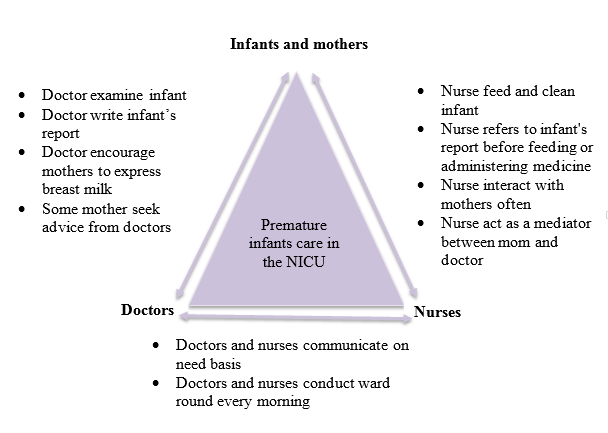
\includegraphics[width=15cm, height=10cm]{Figures/workflow.PNG}
    \caption{Groote Schuur Hospital NICU Workflow.}
    \label{fig:workflow}
    \end{figure}

We identified that the infants are fed in four-hour intervals, a schedule that nurses adhere to ensure that the health of the infants improve. The nurses use the feeding and medication instructions issued by the doctors. While conducting our volunteer work, nurses informed us that breastfeeding is critical to premature infants’ recovery and mothers are sensitized to express enough milk for their infants~\citep{Kapembwa2017, Updegrove2013}. Without this, infants fed on formula milk are at the risk of developing Necrotizing Enterocolitis (NEC); a disease that affects the intestine of premature infants in the second to third week of their life ~\citep{Updegrove2013}. 

We recognised that communication is essential while taking care of premature infants. Doctors and nurses interact often when conducting medical procedures on infants in the ward to ensure that they are in the same page in terms of the infants' condition and the treatment. Nurses consult the doctors before administering medication or discharging/moving an infant from the unit. On the other hand, doctors consult each other often and sometimes they use the neonatal medical book or use their phone to access online medical information when conducting procedures and writing medical reports.  

However,there is minimal communication between the NICU staff and mothers of premature infants.  A number of researchers have documented this finding ~\citep{Griffin1998, Pascoe2016, Jones2015}. From our observation and interview sections we identified that the nurses interact with mothers only when training them on latching and skin to skin care. The main reason for these minimal interactions is because the NICU staff are constrained by a heavy workload. As a result, they rarely interact with mothers to offer psychological support. This finding resonates with prior studies that  reveal that  mothers are prone to stress due to lack of regular and informative communication with the NICU staff ~\citep{Orzalesi2011,HadianShirazi2015, VandeVijver2015}. This was one of the motivation that made us focus on understanding the essential information that mothers need so that they can understand their infants’ condition and health progress. To further investigate the needs of the mothers, we opted to observe all the sections in the unit both during the day and night.  

\subsection{NICU Environment}
Groote Schuur Hospital NICU is equipped with incubators, monitors and other machines that are used to care for sick premature infants. The unit is small with incubators placed close to each other with plastic seats in between the incubators. To prevent overcrowding, the unit restricts visits to parents and grandparents of sick infants. However, during interview sessions, mothers mentioned that they would appreciate if visitors---especially their spiritual leaders, were permitted to visit and conduct prayers for their hospitalized infants. To clarify why such visits are discouraged, one nurse shared the following anecdote:

\enquote{\itshape We once had an incident where a spiritual leader applied oil on the infants face which is not allowed because infants' skin is sensitive. The same oil could be a potential source for spreading germs because of its application on other users outside the NICU}. 

During the day, doctors and nurses conduct rounds in the unit at around 11 a.m. Doctors have a responsibility of providing medical reports of all infants under their care. Their discussion happens around infants' incubators and mothers are seldom included in these discussions. One mother mentioned:
\enquote{\itshape The doctors would only ask me how I am doing and continue with their conversation like i was not there.}
NICU staff revealed that language barrier is the main hindrance to mothers engagement in these discussions. To affirm this claim, majority of the mothers said they could not understand the accent of the doctors and they required nurses assistance to interpret the information on infants' progress report book. In addition, technical medical terms are often used and mothers barely understand them. Instead, mothers usually nod in agreement despite not understanding what the NICU staff are talking about.

At night, there are few mothers in the NICU. Mothers and their partners are allowed in the unit until 8 p.m. There are few nurses at night and they work round the clock to ensure infants are fed and cleaned on time. Only one doctor is on call to handle emergency cases. Both doctors and nurses conduct rounds in the unit to ensure NICU equipment connected to the infants are operational. Next, we provide and discuss detailed activities of each section in the unit. 

\textbf{ICU1 Section:} ICU1 admits critically ill infants who are referred from other hospitals in Cape Town or newborns from the GSH labor ward. These infants are always under supervision to ensure that they breathe normally through the support of machines. Doctors in this section work closely with the nurses to confirm the infants receive the correct amount of oxygen and medication. There are few mothers in this section. Reason being majority of them are still recovering in the obstetric ward and are not able to frequently visit the section. 

The admitted infants are tiny and their sight is traumatizing. Mothers mentioned that they were uncertain of their infants' survival based on their small size and weight. They relied heavily on NICU staff to support them during this challenging times. Similarly, the sight of the infants had the same effect on the researcher. As acknowledged by (Moncur, 2013), it is important for researchers conducting sensitive study to have support mechanisms in case they become distressed or troubled by their research. To adhere with this practice, we sought psychological support from the senior nurses at the unit who oriented us to the section daily activities such as minor operations, blood transfusion and occasionally resuscitation. This helped us to understand and familiarize ourselves with the workflow and activities of this section. The nurses also advised us to focus on other sections since we were not comfortable with the intense medical activities in ICU1. We only spent three days in this section and focused on other sections as advised by the nurse.

\textbf{ICU2 section}: The ICU2 section is located opposite the ICU1 section. In between these two sections, is the working station where nurses and doctors handle NICU related phone calls. Similar to ICU1, this section admits critically ill infants whose breathing is supported by machines. Contrary to ICU1 section, in ICU2, there is presence of mothers accompanied by their partners who offer them support as they strive to adapt to the NICU environment and motherhood in general. Majority of these mothers remain admitted in the obstetric ward and they visit this section to deliver their expressed breast milk. They seemed to be in pain and as they were still recovering from cesarean childbirth. Also, we observed that most mothers struggle with breast milk expression and occasionally they requested for nurses assistance. Due to nurses heavy workload, they handed over pamphlets to mothers and asked them to learn milk expression from the instruction provided. Due to insufficient support, these mothers sit next to their infants’ incubator and cry as they attempt to express enough breast milk for their sick infants. During interviews sessions, mothers confirmed they were distressed by the sight of their infants connected to numerous devices and cables, for which they did not understand their functions. 

In addition, they mentioned that the NICU environment in general was terrifying. This confirms \textcite{Obeidat2009} claim that NICU environment is intimidating thus causing significant level of stress on mothers. Mothers mentioned they are afraid of touching their infants lest they disconnect the cable attached to them. In addition, the alarms of the display machine connected to the infants kept going off, thus agitating new mothers in the section. At one instant, we saw a mother calling out the nurses when the alarm connected to her child's display machine started blinking. The nurse switched off the alarm without informing the mother what triggered the alarm. The nurse checked the infant and told the mother that everything was fine with the infant. When the alarm went off the second time, the same mother switched off the alarm without consulting the NICU staff. This was common among mothers in this section. The nurses informed us that the alarm sometimes are triggered by frequent touching of infants which interferes with infants' thermal regulation. This case is not critical, though they mentioned that the machine calibration needed to be reset to fix some of the false alarms. The nurses' remarks thus explained why we observed fewer alarms at night.

 \textbf{High care 1 and high care 2 sections:} The High care 1 and high care 2 sections admit infants with chronic illness. These infants can stay in these sections up to three months. There are numerous mothers during the day who visit the unit on a daily basis to nurse their infants. These mothers come in the morning with a jar of expressed breast milk. First thing, they label the jar with a sticker and store it in the refrigerator. Then, they sit next to their infants’ incubator and continue expressing more breast milk or they conduct skin to skin care. Mothers said they liked holding their infants in their arms to forge mother-infant bond. To encourage mother-infant bond, nurses inspired mothers to take up their maternal role by training them to cup feed, clean and hold their infants close to their skin. Although mothers were expected to visit the unit everyday, we noticed some mothers occasionally visited their infants. In cases where a mother did not visit the unit for two consecutive days, nurses used landline phone to ask them to deliver expressed milk to the hospital. Infants who were rarely visited were fed on formula milk, exposing them to gastrointestinal infections which has an effect of slowing their development \citep{Embleton2001}. \enquote{\itshape We always make an effort to educate mothers on the importance of breastfeeding}, said the nurses. They intervene by giving mothers pamphlets which list the benefits of breastfeeding. The pamphlets are usually in English, isiXhosa and Afrikaans language.

Despite nurses intervention, mothers who are new to the unit appear to be lonely. In one instance, a mother was seen calling out a nurse to help her with milk expression. The nurse gave her a pamphlet and asked her to follow the instructions before resuming on her busy schedule. The mother appeared frustrated because she was not able to express any milk despite following the instructions. \enquote{\itshape The NICU staff are always busy with minimal time to interact with us},mothers affirmed. As a result, mothers tend to consult each other. During our observation sessions, we viewed them trying to interpret the medical reports of their infants. They also shared their personal information and encouraged each other the best they could.

However, majority of mothers are afraid to approach the doctors. During the ward rounds, mothers tend to be more of observers and they seem not to understand their infants' development status. In one instance, a mother was asked whether she understood the condition of her infant. \enquote{\itshape I can not understand the medical terms contained in my infant’s progress report}, she said. The consultant asked one doctor to explain the condition in simple terms but eventually, the conversation ended up being complex thus leaving the mother out of the conversation. Eventually, mothers opt to follow up on the ward round conversation by approaching nurses who can communicate in their vernacular languages. In the case where nurse are not able to interpret medical information, they involved doctors in the conversation, as they act as information mediators. 

\textbf{Kangaroo Mother Care (KMC) section:}
The KMC section admits infants with stable health who awaits to be discharged. Mothers in this section are familiar with the NICU environment after being there for more than one month. However, there are new mothers in this section who need constant assistance from the NICU staff. There is staff shortage and only three nurses and one doctor are allocated in this section. These NICU staff are overwhelmed with the workload and we noted that infants cry longer before they are attended to. In some instances, we observed nurses giving syrup to crying infants to sooth them to sleep so that they could continue with their daily role. In addition, the alarms go off quite often and they remain unattended for a longer time than in other sections. 

There are few mothers in this section. This is because mothers are aware of their infants' stable health and they await to be discharged. Nurses confirmed this when they said:

\enquote{\itshape Mothers whose infants have been admitted in the NICU for a long time feel relieved when their infants are transferred to the KMC section. They are assured they will be going home soon}. 

Also, one mother mentioned:

\enquote{\itshape My child had breathing issues for two weeks. I got relieved when i found nurses had moved her to the KMC section}.\bigbreak

KMC is generally the last section an infant goes through on their path to recovery and discharge. Mothers visit the section only when they are delivering expressed milk for their infants. For mothers who are unable to commute frequently, the hospital has set aside a small room in this section where mothers can board.

Unlike in other section, mothers in this section were familiar with breast milk expression and conducting skin to skin care. They required minimal assistance from the nurses as they cared for their infants. These mothers have learned the habit of switching off alarm without consulting the NICU staff. Majority of mothers mentioned: \enquote{\itshape I saw other mothers switching off the alarm and I decided to do it as well.} Nurses are mostly busy and have no time to attend to the alarms. Instead, they focus more on infant feeding and hospital transfer or discharge planning. Due to lack of sufficient information, mothers are not equipped to engage in the decision making of their infants health and care of their infants. As a result they feel like they have lost their maternal role which often make them worried and anxious thus exacerbating their level of stress. In the next session we discuss factors that we identified as the major cause of stress among mothers of hospitalized premature infants.

\subsection{Source of Stress In the NICU}
Premature delivery and hospitalization are stressful events for mothers \citep{Wigert2012, Heidari2017}. Our stakeholders confirmed that NICU environment is stressful for everyone. Mothers mentioned that they didn't expect to deliver prematurely since they routinely attended antenatal appointments. Therefore their infants admission in the NICU was unexpected and traumatizing. All the same, five mothers (two were hypertensive and three diabetic) mentioned that doctors had prepared them psychologically and they were aware of possibilities of premature birth. From our interviews session we identified and categorized the common sources of premature relate birth stress into four groups as discussed below:

\subsubsection{Infant’s Health Condition}
The main cause of premature-related stress is the uncertainty of infants' health condition. All mothers mentioned that their infants health was unpredictable since infants' condition fluctuated quite often. For instance, one mother said:

\enquote{\itshape Each and every day, my child was on a different type of oxygen and I did not understand why his health was deteriorating} \bigbreak
Another mother mentioned:

\enquote{\itshape My babies weight was low and it was not improving. She vomited all the milk she took. She had to be moved from Highcare1 to ICU2 section. This was stressing. I expressed enough milk for my baby but her health was not improving} \bigbreak
Mothers relied heavily on the support they received from NICU staff to manage their levels of stress. However, NICU staff have minimal time  in their schedule to provide psychological support to mothers. In stead they work round the clock to ensure that the infants are fed and cleaned. On the other hand, mothers are unable to understand the medical terms used when NICU staff share infants' health update with them. To handle this challenge some mothers, opt to befriend nurses who speak their vernacular language to receive frequent updates on their infants' health status. Foreign mothers and those who are unable to speak South Africa common languages always feel out of place and helpless.
 
\subsubsection{Economic Factors}
Mothers whose infants are admitted to GSH NICU are mostly from low-income communities around Cape Town. Majority of them are single parents and they receive support from their parents and the South Africa government social funds. All of them encountered financial challenges during their infants hospitalization. \textcite{Blencowe2013} review of epidemiology of preterm birth shows that the cost related to neonatal intensive care are high and they place additional burden on families resources. We confirmed this finding as we interacted with mothers who participated in this study. They mentioned that they incurred high high transport cost---which they had not budgeted for, whenever they travel to the hospital.

\enquote{\itshape I had not budgeted for the travel cost and i used a lot of my saving on taxis. I had to skip hospital visits whenever  i did not have money, although I did not feel comfortable being away from my child} \bigbreak
We also identified that three mothers had to quit their job to take care of their hospitalized infants. They were not entitled to maternity leave thus leaving them with no option but to quit their jobs. Consequently, they encountered financial challenges which affected them emotionally because they could not provide basic needs to their families. One mother commented :

\enquote{\itshape I had other children back at home and I was torn between taking care of the family back at home and visiting the sick child in the NICU.}

\subsubsection{Social-Cultural factors}
11 out of 15 mothers related their premature birth and hospitalization to their various cultural beliefs. Separation and reduced opportunities to interact with their infants are against their culture and they felt they were not fulfilling their maternal role. Also, they attribute their premature birth to certain cultural practices they failed to conform with while pregnant. For instance, one Xhosa woman said:
\enquote{\itshape I didn't follow the Xhosa cultural practice when I was pregnant and I sometimes think that's what caused the early birth. In my culture, we must follow the cultural practice to prevent evil spirits from attacking the fetus.}
 In addition, religion and spiritual practices, served as a background to explain the present condition of their infants. These sample of comments expresses mothers views:
 
\enquote{\itshape I believed that my child would get well if the Imam prayed for him. Unfortunately, the Imam was only available at night and the NICU would not allow visitors past 8 p.m. I was depressed and I felt like my child's health was deteriorating because we did not conduct the prayers.} 

\enquote{\itshape I believed that if my pastor anointed my child, he would have gotten better quicker}
From the interviews, we identified that mothers incorporated their cultural beliefs while providing care to their infants. We comforted the mothers by educating them on possible causes of preterm births. We also informed them that preterm birth can happen to anyone and it is not related to any cultural practices. To reiterate on this information we asked mothers to further consult clinical information pertaining causes of preterm births from nurses who were familiar to their cultural practice.

\subsubsection{Insufficient Communication} 
Lack of supportive and up to date neonatal information emerged as the major cause of stress among mothers of preterm infants. 13 mothers, felt like the nurses had taken up their parental role and they were not involved in their infants' health decision making process. For instance, one mother said:

\enquote{\itshape I was admitted to the obstetric unit and when I went to visit my baby in the NICU, I found my child being fed with formula milk. I was angry because no one had asked me for my breast milk} \bigbreak
Another mother mentioned:

\enquote{\itshape My child was moved from ICU2 to high care1 section and I was not informed. I had to walk in the NICU thinking the worst had happened to my child but I later found her.} \bigbreak

They mentioned that they needed emotional support from the NICU staff to help them cope with their infants, illness and other aspects of the NICU environment. Akin to \citep{Axelin2006} study, mothers wanted detailed information of the NICU procedures that staff conducted on their infants to help them manage the stress related to painful situations of their infants. Two mothers mentioned that they say doctors drawing blood from their infants' and they could not stand the sights because their infants were crying loudly.

\enquote{\itshape They did not tell me what they were doing to my child and I felt helpless because I could not protect him from pain}\bigbreak

\enquote{\itshape My baby cried a lot when they drew blood from her head. They did not tell me what the test was all about and I felt helpless not knowing how to comfort my baby.}\bigbreak

We followed up with the doctors to understand why they did not involve mothers during NICU procedures.


\enquote{\itshape We do not encourage mothers to be around the procedure table because the process is intensive and they always get overwhelmed with emotion thus interfering with the process}\bigbreak


\enquote{\itshape We use simple language to inform mothers about the procedures but they seem not to understand. }\bigbreak
Also, mothers mentioned that the NICU environment is filled with unfamiliar equipment which they are never oriented on once their infants are admitted in the NICU. They fear touching their infants lest they disconnect cables connected to them. In addition, the alarms in the NICU keep going off and mothers are not sure what triggered them. They reiterated that it was important to be oriented to the NICU environment and equipment to help them familiarize with the environment. 


Based on these responses, we concluded that there is communication barrier between staff and mothers. Similar results were reported by \citep{Mok2006, Aagaard2008}. Ineffective communication between staff and mothers strains their cooperation in infant care thus aggravating mothers stress levels. Mothers want frequent communication with staff which included chats, encouragement and general talk about premature birth. However, NICU staff mentioned that the NICU has shortage of staff and they work round the clock to ensure that the infants health stabilizes thus neglecting the emotional needs of mothers. Consequently, mothers,struggle with sharing the care of their baby and in building strong relationships with NICU staff. They avoid voicing their issues in fear that this might make them appear as difficult mothers which in turn may stop the staff from tendering to their infants. To enable the reader to understand the communication challenges in the NICU, we will categorize NICU communication into three groups and discuss them in the next section.

\subsection{Communication in the NICU}
The care of premature infants involves different stakeholders who need frequent sharing and discussion of information related to infants' health status~\citep{Wigert2014b}. Effective communication among the NICU staff, and between the NICU staff and the parents is essential for informed decision making and parental satisfaction~\citep{Kowalski2006}. Based on our observation and interview sessions, we identified three categories of  NICU interaction. These are Communication between: 1. NICU staff 2. NICU staff and mothers and 3. mothers. 

\textbf{Communication between NICU Staff:}
The nurses, doctors and the NICU clerks work closely to ensure that they are in the same page in terms of infants health status. In the morning at 7 a.m when the day shift nurses report at work, they take a ward round with the night shift nurses who update them on the health status of each infant. Infant information is recorded in each infant's progress report book which is placed on a tray beneath the incubator. Similar communication happens in the evening at 7 pm when the night shift nurses arrive.

During the day, doctors and nurses conduct a ward round at 11 am. Doctors give a report of each infant’s health condition and progress to the team. At the same time, nurses take notes to record health condition of each infant. We identified that most of the communication during the ward round is between doctors. Nurses were only involved when they needed to specify the amount of feeds and medication administered on infants. Hence, we established that communication between doctors and nurses were few and they happened on need basis. During the day the main conversations between doctors and nurses is around the infant feeding, medication and hospital discharge/transfer information. Nurses consult doctors when they need clarification on feeding or medication information. During section transfer or hospital discharge, nurses must consult the doctor before the infant leaves the section.

Moreover, we identified doctors and nurses have separate reporting books and meetings which are held at different days of the week. Nonetheless, the doctors do invite nurses in their weekly meeting which is held every Friday at 11pm. During the day the main conversations between doctors and nurses is around the infant feeding, medication and hospital discharge/transfer information. Nurses consult doctors when they need clarification on feeding or medication information. During section transfer or hospital discharge, nurses must consult the doctor before the infant leaves the section. 

Nurses work together to ensure that the infants are fed and cleaned at the scheduled time. They consult each other before administering medication. For instance, we observed two nurses using a calculator on their mobile phone to calculate the drug dosage. On follow up, we learned that they use calculator to ensure infants receive the correct dosage to avoid further complication. To ensure smooth running of NICU workflow, they take tea and lunch break in intervals. Before a nurse leave the unit, they have to alert others so that all NICU sections are covered throughout the day.

On the other end, doctors interact among themselves when they are conducting procedures or when discussing infants’ health condition. They meet around infant incubators and discuss infant’s diagnosis. Although, they rarely include mothers in these conversation. Often, doctors work individually in their allocated part of the section.

\textbf{Communication between NICU staff and mothers:}
Communication between mothers and their infant’s principal medical care providers is important in the NICU setting. It ensures that mothers are involved in every decision made on their infants’ health \citep{Orzalesi2011, HadianShirazi2015}. It is important for mothers to freely communicate with staff in the NICU to understand their infant’s condition, participate in medical decision making and  partake in the care of their infants~\citep{Wigert2014b}. However, we identified there is minimal interactions between the staff and the mothers--- especially those between mothers and doctors. 

\enquote{\itshape We have a heavy workload and rarely have time to support or interact with mothers}, doctors confirmed. They are overwhelmed with their daily NICU duties thus leaving them with little time to interact with mothers.

Nurses often interacted with mothers who are new in the NICU to educate them on breast milk expression, cup feeding and skin to skin care. This initial interaction is brief and the nurses subsequently give mothers pamphlets to complement their interaction. Nonetheless, they follow up on mothers who face lactating challenges to educate them on breastfeeding diet. Also, they interact with surplus breast milk to encourage them to donate to the hospital milk bank that support infants whose mothers are not able to express enough breast milk. Although nurses strive to support mothers, they mentioned that some mothers do not comply with the advise provided. For instance, we observed a mother being scolded by a nurse because she had not delivered expressed milk for her baby. The nurse said:

\enquote{\itshape Your baby is sick and vomiting because you don’t want to express milk. Formula milk is not good for your baby and you are not putting any effort to help her}\bigbreak

Nurses said that they are sometimes demanded to be harsh on the mothers to ensure that they cooperate in infant care. As a result, mothers fear them and comply to their request to avoid being rebuked. 

For mothers who are concerned with their infants health status and development, NICU staff often prioritize on providing them with infants' up to date information. They use layman's language to explain infants' condition to mothers. Even so, some mothers are not able to understand medical information pertaining their infants. This is either because they fear asking questions or they do not understand English. The staff said infants health is unpredictable and they often provide mothers with accurate information to calm their anxiety. Although worrying and anxiety are sometimes unavoidable among mothers, doctors try their best to offer psychological support when needed. 

\enquote{ \itshape I pay close attention to maternal instincts. I believe mother-child's bond is strong and if a mother insists that I should check on her baby, I do it immediately because their intuition may be suggestive of child’s health condition}, disclosed a doctor. \bigbreak

Over all, there is minimal interaction between doctors and mothers in all sections of the unit. During the ward rounds, doctors initiate conversation with the mothers but they seem not to understand the shared information. Mothers often nod in agreement to everything said by doctors but when asked to explain their infants condition based on their understanding, they keep quiet or sometimes confirm that they do not understand the medical terms used. Most mothers are afraid to initiate a conversation with the doctors and they mainly rely on nurses to connect them with the doctors.

\textbf{Communication between mothers:}
Mothers interactions are common in HC1, HC2 and KMC sections. Majority of these mothers have been in the NICU for more than two weeks and they appear to be familiar with each other. They sit close to each other and chat about their infants' health and personal information. All mothers commended these interactions saying that they were supportive and necessary especially when a mother is new in the NICU. We established these mother-mother interactions played a  peer-support role as well as an encouragement channel for mothers in the NICU. One mother confirmed this when she said:

 \enquote{\itshape I talked to a mother who told me that her son had the same condition as my baby and he was fine after two weeks. This was encouraging and it helped me to stay positive}

Another mother who was new in Cape Town said:

\enquote{\itshape I did not know anyone in Cape Town and mothers in the NICU supported me emotionally and financially. They contributed money for my bus fare when my baby was discharged}

Majority of mothers mentioned that interaction with other mothers helped them to cope with stress related to premature birth. All the same, there were mothers who preferred being alone. Most of these women were from foreign countries and thus they were unable to communicate in English or common South Africa languages. We observed them crying as they watched their infants in the incubators. Occasionally the nurses would sit next to them and comfort them. 

Despite these interaction being helpful, mothers insisted that there was a need of frequent conversation with NICU staff to help them partake in the decision making of their infants' health. This verified our observation in HC1 and HC2, where we saw mothers asking for nurse assistance as they attempted to interpret the medical information on the infants' progress report. Over all, NICU interactions helped us to understand the communication gaps and how the stakeholders attempt to cooperate in infant care. So how does the NICU staff augment NICU communication? Below, we discuss some of the technological intervention that the NICU use to relay information to mothers.


 \subsection{Technological Intervention Used to Support NICU Communication}
During our observation session, we identified NICU staff and mothers use technology quite often. Doctors use the mobile phone to communicate among themselves in the unit. For instance, we observed a doctor using mobile phone to call another doctor based in another section of the unit to consult on a certain infant’s health condition. Eventually the other doctor came  to first doctor working station. They use both neonatal medical book and online medical information (viewed via mobile phone) while conducting medical procedures on infants.

However nurses are not allowed to use mobile phones while in the NICU:

\enquote{\itshape We are not allowed to use our mobile phones in the unit.We have to pick or make personal call outside the unit}, said nurses. \bigbreak

This rule is implemented to reduce the spread of germs and infection in the unit. However once in a while we observed senior NICU nurses using mobile phone calculator to get accurate measurement of medication. This is allowed in the unit as long as nurses sanitize their phones before using them in the unit. Also they have to sanitize their hands before coming in contact with infants.

As for mothers, we learned that they often use their mobile phones to communicate with their families and friends. 11 mothers owned smartphones and they sometimes use them to access social media such as WhatsApp and Facebook.
\enquote{\itshape the data cost is so high and we only buy it when we need to relay important information to our friends and families} \bigbreak
They mostly use their phones when they are conducting skin to skin care. To avoid distracting other people int he unit, they use earphones to listen to music as they scroll through social media sites. They also used their phones to take photos of their infants to keep track of infants’ development progress. 

Through the interview sessions, we identified that most mothers at the unit rarely use technology to access information related to their infant’s health. Instead, they feel guilty for not carrying their infants to term and use mobile internet to identify factors that could have led to a premature birth. 12 mothers reported having used the internet during their pregnancy to access pregnancy and motherhood information. Only 3 mothers used the internet to access premature birth-related information. 

\enquote{\itshape The online information is unreliable and I chose to rely on information provided by the NICU staff}, said a mother.

Overall our baseline study demonstrates that NICU staff use technologies such as text messages and phone calls to communicate with mothers. However, these interventions provide limited opportunity for comprehension support. For instance, the phone call mode has shortcoming such as delays in connecting to the hospital switchboard, inaccessibility of mothers who have changed their phone number etc. In addition, the mothers mentioned that it was expensive to call the hospital and this hindered them from getting updated medical status of their infants.

All NICU staff said: \enquote{\itshape mothers change their phone number quite often thus it is hard to get hold of them when we call them sing the units landline phone} 

Also some mothers share their phones in their household and due to the health information confidentiality in the unit, NICU staff are restricted from sharing infant information with any other person apart from infants parents.

\enquote{\itshape  Some  mothers share their partners phone number. Since they are not legally staying together, we are do not share any information with them. Instead we ask them to inform mothers to call the unit}- nurse

However calling the unit phone is expensive because mothers call were directed to the hospital switchboard before being redirected to the units phone.

\enquote{\itshape You could wait for up to 10 minute before you speak to nurses in the NICU. I tried once and opted never to do it again}

Literature shows that technology interventions have the potential to increase communication between mothers and the infant’s care team, potentially reducing maternal stress and improving understanding of infant's condition \citep{Garfield2016, Weems2016}. Although technological intervention can improve communication, they should not replace the one-on-one communication between mothers and staff in the NICU. However in GSH NICU context it was clear that technological interventions were not effective in alleviating mother level of stress. We then followed up with our participants to determine potential cost saving strategies for bridging communication in NICU.

\subsection{Participants' Perceptions Towards the Use of Technology in NICU}
During interview sessions, we investigated participants views on use of technology to enhance NICU communication. Based on our thematic analysis we identified three categories of information that both NICU staff and mothers preferred to be shared via technological intervention. These are: 1. Breastfeeding information 2. Infants health status 3. Intersection transfer and hospital discharge information. The table below summarizes the need and possible technology that could be used to relay this information.

\begin{table}[h!]
\caption{Suggested Technologies that can be used to relay Information}
\label{tab:perceptions}
\begin{tabular}{|p{2.5cm}|c|c|p{4.5cm}|}
\hline
\textbf{Information} & \textbf{Technologies Suggested by Participants} \\ \hline
Breastfeeding information & \begin{tabular}[c]{@{}l@{}}Digital video to educate mothers on breast milk expression\\ Text messages to remind mother to deliver expressed breast milk\\ Interactive website\end{tabular} \\ \hline
Neonatal information & \begin{tabular}[c]{@{}l@{}}Text messages to inform mothers on infants' health\\ Toll free number that mothers can call to inquire on infants health\\ Digital video explaining common medical conditions\end{tabular} \\ \hline
Infant hospital transfer information &Text message to inform mothers on infants' hospital transfer \\ \hline
\end{tabular}
\end{table}

We learned these are categories of information that mothers often enquire from NICU staff. Currently, this information is only available to mothers who are present in the NICU thus leaving out mothers who are unable to visit the unit on a daily basis or those who are afraid to approach NICU staff in the unit. Participants acknowledged that majority of mothers owned phones. However, they were adamant that the process of accessing information should not involve any data costs. Consequently they suggested cost effective strategies for disseminate information.

In the interview sessions, we confirmed that mothers of premature infants experience numerous lactating challenges. Mothers proposed that they would like to access educative information that could encourage exclusively breastfeeding. In addition, nurses suggested that mothers needed to be educated on breast milk donation--- a concept that is encouraged in the unit to aid infants whose mothers are unable to breastfeed their infants. These statements confirm their suggestion:

\enquote{\itshape We can use text messages to educate mother on benefits of breastfeeding and also the concept of breast milk donation}\bigbreak

\enquote{\itshape First time mothers and teenage mothers have lactating issues and they require frequent support. With availability of mobile phones, they can easily access lactating information and essence of breast milk donation}\bigbreak

We interrogated them further to find their perceptions on possible technological strategies that could be used to access the suggested information.they provided numerous suggestion which we coded them into three: 1. digital videos 2. text messages and 3. interactive website.

In terms of neonatal information, mothers mentioned that they needed frequent updates of their infants health status. Contrary to the mothers, NICU staff reiterated that due to health information confidentiality, it was impossible to share neonatal status via mobile phone. Instead, they recommended that text message could be used to inform mothers to visit the hospital immediately in case of emergencies. On the other end, mothers, suggested use toll free number that  mothers who are unable to visit hospital frequently could use to inquire on their infants help status. For those who are available in the NICU, both staff and mothers unanimously said they could use digital videos to learn on their infants health conditions.

Additionally, mothers wanted to access information on their infants inter-section and hospital transfers. Mothers used their NICU experience to justify why this information was necessary. For example one mother said:

\enquote{\itshape  I visited the unit and found they had moved my baby from the section i had left her. They did not inform me about it and i had to move around the NICU to look for her} \bigbreak

Unanimously, NICU staff and mothers proposed the use of text messages as the most appropriate mode of sharing updates on infant transfers.

\section{Discussion and Implication for Design}
In this section, we discuss the lessons we learned as we focused on understanding the NICU context, our participants and their perceptions in terms of suitable technological interventions that could enhance NICU communication.

\subsection{ Empathy's Role in Understanding Participants}
Empathy-building is essential in the initial phase of co-design process in which researcher/designers seek to understand their intended end-users. Empathy is defined as the ability to identify and relate with the feelings or suffering of another \citep{Bennett2019}.  The process of co-design begins with understanding of participants/users, their environment and the problem that you are trying to solve for them. We argue that researchers venturing in under-researched domain such as the NICU should adopt a novice mindset to enable them to understand the workflow and people in totality. Volunteer work in the NICU was one on the most useful aspects of our study. Working in our participants natural environment helped us identify NICU communication channels, staff-mothers interaction and some factors that hindered effective communication. Also, it helped us build rapport with nurses who we eventually worked with throughout the study. Although we were the research lead, we acknowledged that they were expert in this domain thus we worked under their supervision as we gradually introduce our research objective to them. 

In this phase, we adopted the research approach that refrained us from assuming NICU communication needs. Instead, we  put aside our presumptions and chose to gain insights from the participants. we opted to listen and observe participants to develop the virtues of our participants by bringing us closer to their NICU experiences. Similar to \citep{Taylor2011}, we assert that HCI researchers should avoid framing and imposing research problems on their participants based on their own theories and limited understanding of the context. Rather, they should immerse themselves in the field work to have a first hand understanding of their participants and their needs. This approach encourages relationship and trust building which is paramount in co-design process. Moreover, it assist in revealing participants nuances of different experiences, needs and aspiration. 

We learned through our interview sessions that we had to foster an empathic disposition to encourage participants to speak openly about their NICU experiences. Being in the hospital environment encouraged our participants imagination thus enabling us to visualize their experiences in their physical environment. Although this sessions were emotionally charged, we focused on ensuring that our interactions did not cause any harm on participants---especially mothers. On the flip side, the interviews sessions took an emotional toll on us and we had to change the topic to help us deal with our own feelings. This emotional event was important in creating rapport with the respondents. It helped us negotiate power imbalance between participants and ourselves as researcher thus encouraging participants to open up about their lives. 

Also, each interview was a mutual educational process. Participants shared difference NICU experiences and we learned about their NICU challenges, culture and their infants, and they learned about various technologies that are currently used to support mothers, our culture and research objectives. We argue, therefore, that researchers conducting sensitive research should not hide their emotional experiences with the participants. Instead, they should use emotions as resources for building rapport with respondents. Consequently, this will help them to have a deeper understanding of their respondents.

\subsection{Ineffective Communication Channels in the NICU}
It was evident that communication in the NICU was fragile, a finding consistent with similar research \citep{Flacking2007,Enlow2017, Wigert2006}. NICU staff work round the clock to ensure that infants health is stable thus neglecting mothers' emotional and psychological needs. Mothers on the other end, expect frequent interactions with NICU staff to help them: understand their infants' development progress, partake in their infants' care and health decision making. However, this rarely happens due to various organisational and communication challenges. Consequently, mothers experience a disconnect in caring for their infants causing a roller coaster emotion among them, which often affect mother to infant bond.

Unlike in \textcite{Turner2015, Wigert2014b}, mothers at GSH NICU are afraid of inquiring for help from the NICU-staff to avoid being marked as a "stubborn mother". Instead, they often be-friend nurse--- those who speak their dialect, to access support. These nurses act a mediators of information between  mothers and doctors. This relationships helped mothers to communicate intimate information such as those related to their cultural believes seeing that they understood them. In turn, nurses used their medical knowledge to educate such mothers on common causes of premature births, disconnecting culture taboos and myths as causes of premature birth.

As in other studies \citep{Gallagher2018, Wigert2014b}, our study evidenced that positive experiences with NICU staff gave mothers a sense of significance in the care of their infants. With prolonged stay in the unit, mothers had learned how to initiate conversation with the nurses when they needed assistance either with breastfeeding information or orientation to the NICU equipment. This is contrary to previous studies such as \citep{Fegran2008, Harrison2010} which shows that conversation between mothers and staff diminished as infants' health stabilized. Mothers identified that they were concerned about their infants health as they were transferred from critical NICU sections to the less critical ones. Despite the fluctuating infants health, mothers were keen to know when they would leave the hospital for home. 

NICU-staff mentioned that providing emotional support to mothers of premature infants was challenging. The challenge was heightened when language or cultural difference between staff and mother existed. This situation place both NICU-staff and mothers in an awkward situation where they are unable to converse. Although the hospital has hired interpreters, they are never available in the NICU since their services is needed in the entire hospital. They also use technological interventions such as phone and text messages to communicate with mothers who are unavailable in the NICU. However, these modes of communication are inefficient and costly. In addition they are applicable when relaying alert messages to mothers in case of an emergency or when a mother has skipped visits for more that two days. 

This leaves the NICU-staff with no option but to use pictorial pamphlets to compliment their support. From our interaction with NICU-staff, we concluded that their support to mothers is attributed to their personal ability rather than mandatory organisational role. We affirm this based on the numerous challenges they face yet they still find time in their busy schedule to provide support. Also this statement by one of the nurse confirms our findings.

\enquote{\itshape I was once a mother of premature infant and I understand how much support these mothers need. That's why I find time to support them when I can}


\subsection{Using Participants NICU experiences as a Resource}
Through extensive  participants' interviews, we identified that there was need of using suitable technological intervention to augment NICU communication. Majority of mothers own android phones but they are unable to afford data and talk time. So how can we use Information and communication Technologies to  share information with mothers?

Due to limited exposure to technology, our participants--- especially the nurses and mothers, did not have proper answers to this question. To engage their imagination, we chose to use their NICU experience to trigger possible  suggestions.

\textcolor{red}{\textbf{STOP STOP STOP}}



Summary

In this report, we have presented some of the major causes of stress among women in the NICU and identified that communication between NICU staff and mothers can help reduce this stress. We had three parts of the study to ensure triangulation. Through interviews and observations, we have established a better understanding of patients’ needs and preferences. One consistent observation we found during this study was that there is insufficient communication between mothers and NICU staff. Most mothers would like to have in-depth communication about their infants' health with the NICU staff but this is not always the case. The NICU is short staffed and the medics mainly focus on the wellbeing of infants thus neglecting mothers psychological needs. Technology is currently being used for communication purposes however there are numerous challenges that hinder effective communication using these media. There is need to enhance communication between NICU staff and mothers of hospitalized infants and in the next phase, we plan to generate ideas on how technology can be used in this context.